\section{Data and measurement}\label{sec:data}

\paragraph{Individual data.}
The analysis pools six rounds of the European Social Survey (R6--R11,
fielded 2012, 2014, 2016, 2018, 2021, and 2023) at the individual level.
Integrated face-to-face files are downloaded via the ESS Sikt API under
per-round DOIs (e.g.\ \texttt{ess11e04\_0} for R11 Edition~4.0). The
pooled panel covers $N=276{,}491$ respondents in 36 country codes
across 154 country-years. The analysis sample after listwise deletion
on individual controls and the L2 macro covariates is $N=165{,}969$ in
30 countries and 135 country-years.

\paragraph{Outcome.}
The institutional-trust composite is the per-item z-standardised mean
of three ESS items: \texttt{trstprl} (trust in [country] parliament),
\texttt{trstlgl} (trust in the legal system), and \texttt{stfdem}
(satisfaction with democracy). Sentinel codes ($>10$) are coerced to
missing before standardisation. Standardisation is per item across the
pooled panel, not within country-year, because the multilevel model
needs to retain the L2 and L3 variance that within-cell standardisation
would mechanically zero out. Models on each item separately appear in
Section~\ref{sec:results-robust}.

\paragraph{Individual GenAI exposure.}
Each respondent's 4-digit ISCO-08 occupation is matched to the
ILO--NASK 2025 occupation-level mean automation score
\citep{Gmyrek2025}, which provides means for 427 ISCO-08 occupations.
Two vintages are available: the 2023 GBB scores \citep{Gmyrek2023} and
the 2025 ILO--NASK re-scoring, which incorporates newer model
capabilities and user familiarity. The 2023 vintage is assigned to
R6--R10 (fielded 2012--2021, before the post-GPT-4 GenAI period), and
the 2025 vintage to R11 (fielded 2023--2024). Within-country variation
in $\bar E_{ct}$ therefore comes from two channels: slow occupational
recomposition, and the capability-vintage shift at R10$\to$R11. A
vintage-static robustness check (2025 throughout, in
Section~\ref{sec:results-robust}) isolates the pure occupational
channel.

The individual exposure measure is z-standardised within the analysis
sample for interpretability and to give the random slope on individual
exposure (M4--M6) a comparable scale. Coverage of the ILO--NASK score
table is 83.4\% across the pooled panel; the remaining 16.6\% have
ESS sentinel codes (\texttt{66666}, \texttt{99999}, \texttt{77777})
or fall outside the 427-code ILO--NASK set, and drop from the
exposure-coefficient sample via listwise deletion.

\paragraph{Country-year aggregation and Mundlak decomposition.}
The country-year exposure $\bar E_{ct}$ is the design-weighted mean of
individual exposure within each (country, round) cell:
\begin{equation}
\bar E_{ct} \;=\; \frac{\sum_{i \in (c,t)} w_i \cdot E_{o(i),v(t)}}
                       {\sum_{i \in (c,t)} w_i},
\label{eq:cellmean}
\end{equation}
where $w_i$ is the ESS \texttt{pspwght} and $v(t)$ is the round-vintage
map. Aggregating from individual ISCO-08 codes inside the ESS preserves
the 4-digit granularity of the score, which a Eurostat LFS-based
aggregation would coarsen. The cell mean decomposes into a stable
between-country part and a within-country deviation:
\[
  \bar E_{ct} \;=\;
  \underbrace{\bar E_c}_{\text{between}}
  \;+\;
  \underbrace{(E_{ct}-\bar E_c)}_{\text{within}},
  \quad
  \bar E_c \;=\; \frac{1}{T_c}\sum_{t} \bar E_{ct}.
\]
Including both terms separately in the regression---in place of
$\bar E_{ct}$ alone---lets the between-country slope $\gamma_B$ and the
within-country slope $\gamma_W$ differ. The Wald test of equality is
the substantive Mundlak test \citep{Mundlak1978}. A leave-one-out
variant $\bar E_{ct}^{(-i)}$ excludes the focal individual from the
cell mean and is used in robustness checks to remove the mechanical
correlation with own exposure.

\paragraph{Macro and institutional covariates.}
Country-year macro covariates come from Eurostat: real GDP growth
(\texttt{nama\_10\_gdp}), unemployment rate (\texttt{une\_rt\_a},
ages 15--74), and HICP inflation (\texttt{prc\_hicp\_aind}); each ESS
round is paired with its modal fielding year. Six countries drop from
the macro-controlled models for Eurostat coverage gaps: Israel and
Russia are outside Eurostat; Albania, Ukraine, and Kosovo lack the
harmonised unemployment and HICP series; and the United Kingdom has no
UK-coded annual unemployment observations for the ESS panel period (a
Brexit-era reporting gap). The L3 institutional moderator is the OECD
Employment Protection Legislation index, version~1, regular contracts,
2007 baseline---a pre-period vintage chosen for exogeneity. Twenty-three
of the 36 ESS countries are OECD members with a non-missing 2007 EPL
value; M6 fits on 22 of these 23 (the United Kingdom drops on the same
unemployment gap). Welfare-regime typology follows the Esping-Andersen
tradition \citep{EspingAndersen1990} with a Western Balkans extension
to the Eastern-European class.

Figure~\ref{fig:exposure} plots country-year exposure trajectories and
the static-vintage comparator; the R10$\to$R11 vintage shift appears as
a downward jump in the cross-country mean. Table~\ref{tab:descriptives}
reports descriptive statistics on the M3a analysis sample (the core
within--between model defined in Section~\ref{sec:methods}).

\begin{figure}[!t]
  \centering
  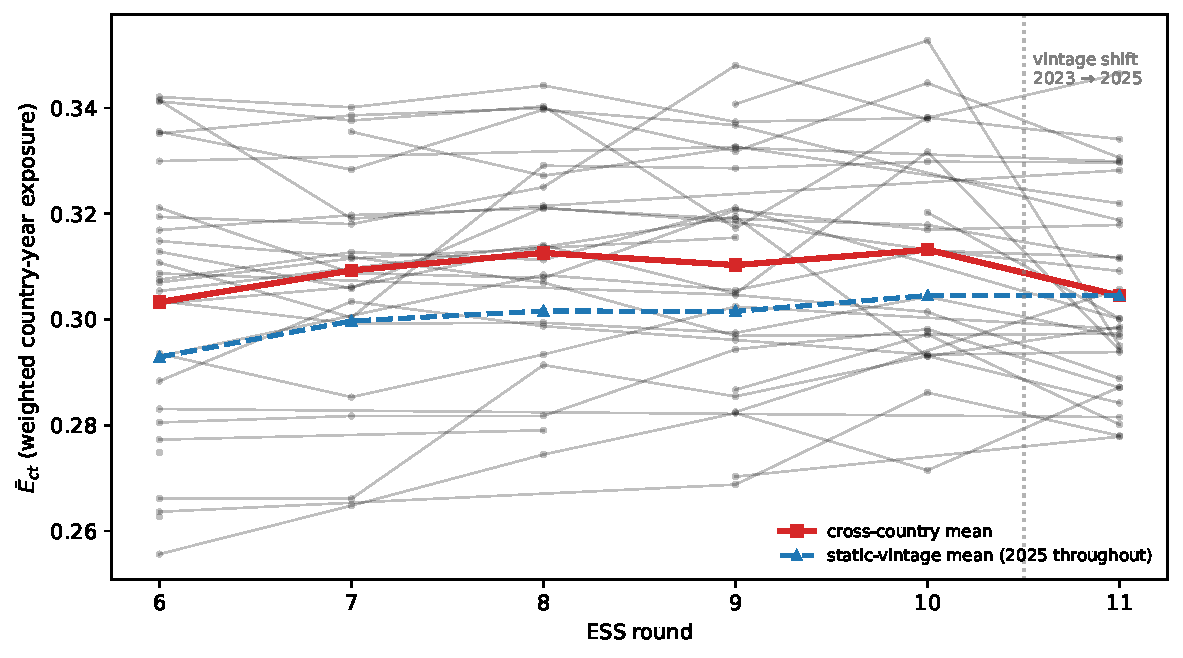
\includegraphics[width=0.92\linewidth]{figures/fig1_exposure_trajectories.pdf}
  \caption{Country-year GenAI exposure trajectories, ESS R6--R11. Thin
  grey lines are individual countries; the heavy red line is the
  cross-country mean; the dashed blue line is the static-vintage (2025
  scores throughout) comparator. The vertical reference marks the
  R10$\to$R11 vintage shift.}
  \label{fig:exposure}
\end{figure}

\begin{table}
\centering
\caption{Descriptive statistics, M3a analysis sample ($N=165{,}969$).}
\label{tab:descriptives}
\small
\setlength{\tabcolsep}{4pt}
\resizebox{\linewidth}{!}{%
\begin{tabular}{lrrrrr}
\toprule
 & Mean & SD & Min & Median & Max \\
\midrule
Trust composite (z) & 0.07 & 0.85 & -2.02 & 0.15 & 2.11 \\
Individual ILO–NASK GenAI exposure (z) & -0.01 & 0.99 & -1.41 & -0.13 & 2.79 \\
Age (years) & 51.67 & 17.36 & 14.00 & 52.00 & 104.00 \\
Female (0/1) & 0.52 & 0.50 & 0.00 & 1.00 & 1.00 \\
Household income decile (1–10) & 5.41 & 2.73 & 1.00 & 5.00 & 10.00 \\
Education (ESS eisced, 1–7) & 4.13 & 1.81 & 1.00 & 4.00 & 7.00 \\
Real GDP growth (\%) & 2.41 & 2.84 & -4.10 & 2.10 & 16.30 \\
Unemployment rate (\%) & 7.58 & 3.88 & 2.20 & 6.80 & 24.80 \\
HICP inflation (\%) & 2.64 & 2.74 & -0.70 & 2.10 & 17.00 \\
$\bar E_{ct}$ (country-year exposure) & 0.31 & 0.02 & 0.26 & 0.31 & 0.35 \\
$E_{ct} - \bar E_c$ (within) & $0.00$ & 0.01 & $-0.02$ & 0.00 & 0.02 \\
$\bar E_c$ (between) & 0.31 & 0.02 & 0.27 & 0.31 & 0.34 \\
\bottomrule
\end{tabular}
}%
\end{table}

